\PassOptionsToPackage{quiet}{xeCJK}
\documentclass{cumcmthesis}
\setCJKmainfont{SimSun.ttf}[AutoFakeBold]
\usepackage{etoolbox}
\usepackage{float}
\BeforeBeginEnvironment{tabular}{\zihao{-5}}
\usepackage[numbers,sort&compress]{natbib}  % 文献管理宏包
\usepackage[framemethod=TikZ]{mdframed}  % 框架宏包
\usepackage{url}  % 网页链接宏包
\usepackage{subcaption}  % 子图宏包
\newcolumntype{C}{>{\centering\arraybackslash}X}
\newcolumntype{R}{>{\raggedleft\arraybackslash}X}
\newcolumntype{L}{>{\raggedright\arraybackslash}X}

\title{全国大学生数学建模竞赛论文模板}  % 论文标题
\tihao{B}  % 题号
\baominghao{202527001171}  % 报名号
\schoolname{西安交通大学}  % 学校
\membera{李冬阳}  % 队员a
\memberb{曹芷维}  % 队员b
\memberc{朱韵桐}  % 队员c
\supervisor{陈磊}  % 指导老师
\yearinput{2025}
\monthinput{9}
\dayinput{7}
\begin{document}


\maketitle

\begin{abstract}
摘要

\textbf{对于问题一,}

\textbf{对于问题二,}

\textbf{对于问题三,}

\textbf{对于问题四,}

最后,



\keywords{关键词\quad  关键词\quad  关键词\quad  关键词 \quad 关键词}
\end{abstract}

\section{问题重述}
\subsection{问题背景}
碳化硅(SiC)作为第三代半导体材料,因其优异的物理与电学性能,在高温、高压、高频等极端工况下展现出巨大潜力。外延层厚度是SiC器件设计与制造中的关键参数,直接影响器件的核心性能指标。因此,建立一套无损、高精度、可重复的外延层厚度测试标准,对产业界与学术界均具有重要意义。

红外干涉法是目前主流的无损检测手段,利用SiC外延层与衬底层折射率不同的特性,发射红外光线并接受来自外延层与衬底层的反射光线,确定SiC外延层的厚度。其基本原理是:红外光在SiC外延层表面与外延/衬底界面分别发生反射,两束反射光因光程差产生干涉条纹,通过分析反射光谱,间接计算外延层的厚度。
%%%%%%%%%%%%%%%%%%%%%%%%%%%%%%%%%%%%%%%%%%%%%%%%%%%%%%%%%%%%% 

\subsection{问题要求}

\textbf{问题1}  
在仅考虑一次反射与透射的简化情形下,建立由红外光谱反演SiC外延层厚度的通用数学模型。

\textbf{问题2}  
利用问题一中我们提出的模型,利用附件1、2中的实测数据计算SiC外延层厚度,并分析结果的可靠性。

\textbf{问题3} 

%%%%%%%%%%%%%%%%%%%%%%%%%%%%%%%%%%%%%%%%%%%%%%%%%%%%%%%%%%%%% 

\section{问题分析}
\subsection{问题一分析}
红外干涉法测量碳化硅外延层厚度的核心在于双光束干涉现象。当红外光以特定入射角照射样品时,在外延层表面与衬底界面分别产生一束反射光。这两束光因传播路径不同形成光程差,其大小取决于外延层厚度、材料折射率及入射光波长。光程差导致两束光在探测器处发生相位叠加:当相位相同时呈现相长干涉(反射率极大值),相位相反时则发生相消干涉(反射率极小值)。

另外,外延层折射率与波长有关。不同波长的入射光在材料中经历不同的折射行为,这使得光程差成为波长的复合函数。这一特性导致反射光谱呈现周期性振荡现象——反射率随波长变化形成明暗交替的干涉条纹,即反射率函数呈现出波动的特性。条纹的振荡频率与外延层厚度直接关联:厚度越大,光谱振荡越密集;厚度越小,振荡越稀疏。

因此,反射率振荡曲线的特征提取是厚度计算的关键。通过分析震荡曲线的特性可建立振荡周期特征与外延层厚度的定量映射关系,即所求数学模型

\subsection{问题二分析}	
对于问题二,

\subsection{问题三分析}
对于问题三,


%%%%%%%%%%%%%%%%%%%%%%%%%%%%%%%%%%%%%%%%%%%%%%%%%%%%%%%%%%%%% 

\section{模型假设}

为简化问题,本文做出以下假设:

\begin{itemize}[itemindent=2em]
\item 假设1 材料均匀:假设外延层是厚度均匀、光学性质各向同性的介质,且其上、下表面是光滑的理想平行平面。
\item 假设2 折射率假设:假设入射介质为空气,其折射率 $n_0$ 恒定为 1。

\item 假设3 光源假设:入射的红外光可视为理想的单色平行光。
\end{itemize}

%%%%%%%%%%%%%%%%%%%%%%%%%%%%%%%%%%%%%%%%%%%%%%%%%%%%%%%%%%%%% 

\section{符号说明}
\begin{table}[H]
\centering
% 修改列数为 4 列,将格式改为 CCCC
\begin{tabularx}{\textwidth}{CCCC}%这里写表格的列数、对齐方式
\toprule
符号    & 说明    & 单位    \\
\midrule
$d$     & 外延层厚度 & $\mu m$ \\
$n$     & 折射率 & 无单位 \\
$\theta$ & 入射角 & 度($^\circ$) \\
$\theta_2$ & 折射角 & 度($^\circ$) \\
$\Delta d$ & 光程差 & $\mu m$ \\
$\lambda$ & 波长 & $\mu m$ \\
$\tilde{\nu}$ & 波数 & $cm^{-1}$ \\
\bottomrule
\end{tabularx}
\label{tab:符号说明}
\end{table}

\section{问题一的模型的建立和求解}
\subsection{模型建立}

$$
E = mc^2
$$

引用公式\cref{eq:公式1}。

\begin{equation}
\label{eq:公式1}
E = mc^2
\end{equation}

引用\cref{fig:山田凉}。

\begin{figure}[H]
\centering
% 修改为指定的 jpg 图片文件名
\includegraphics[width=0.75\textwidth]{未标题-1.jpg}
\caption{单图}
\label{fig:山田凉}
\end{figure}

这句话引用了文献\cite{司守奎2011数学建模算法与应用}。

这句话引用了文献\upcite{卓金武2011MATLAB}。

\textbf{猫猫}尝试两张图搞搞

看起来你输入了“喵”,若你有关于当前打开的 LaTeX 文件的问题,比如解释代码、修改代码、生成新代码等,都能随时跟我说,我会帮你解决。
\begin{figure}[H]
\centering

\includegraphics[width=0.5\textwidth]{mmexport1751906318520.jpg}
\caption{单图}
\label{fig:新图}
\end{figure}

垃圾latex

\section{问题二的模型的建立和求解}
\subsection{模型建立}

引用\cref{fig:双图},引用\cref{fig:双图a},引用\cref{fig:双图b}。

\begin{figure}[ht]
\centering
\subcaptionbox{双图a子标题\label{fig:双图a}}
{
\includegraphics[width=.4\textwidth]{mmexport1751560996590.jpg}}
\subcaptionbox{双图b子标题\label{fig:双图b}}
{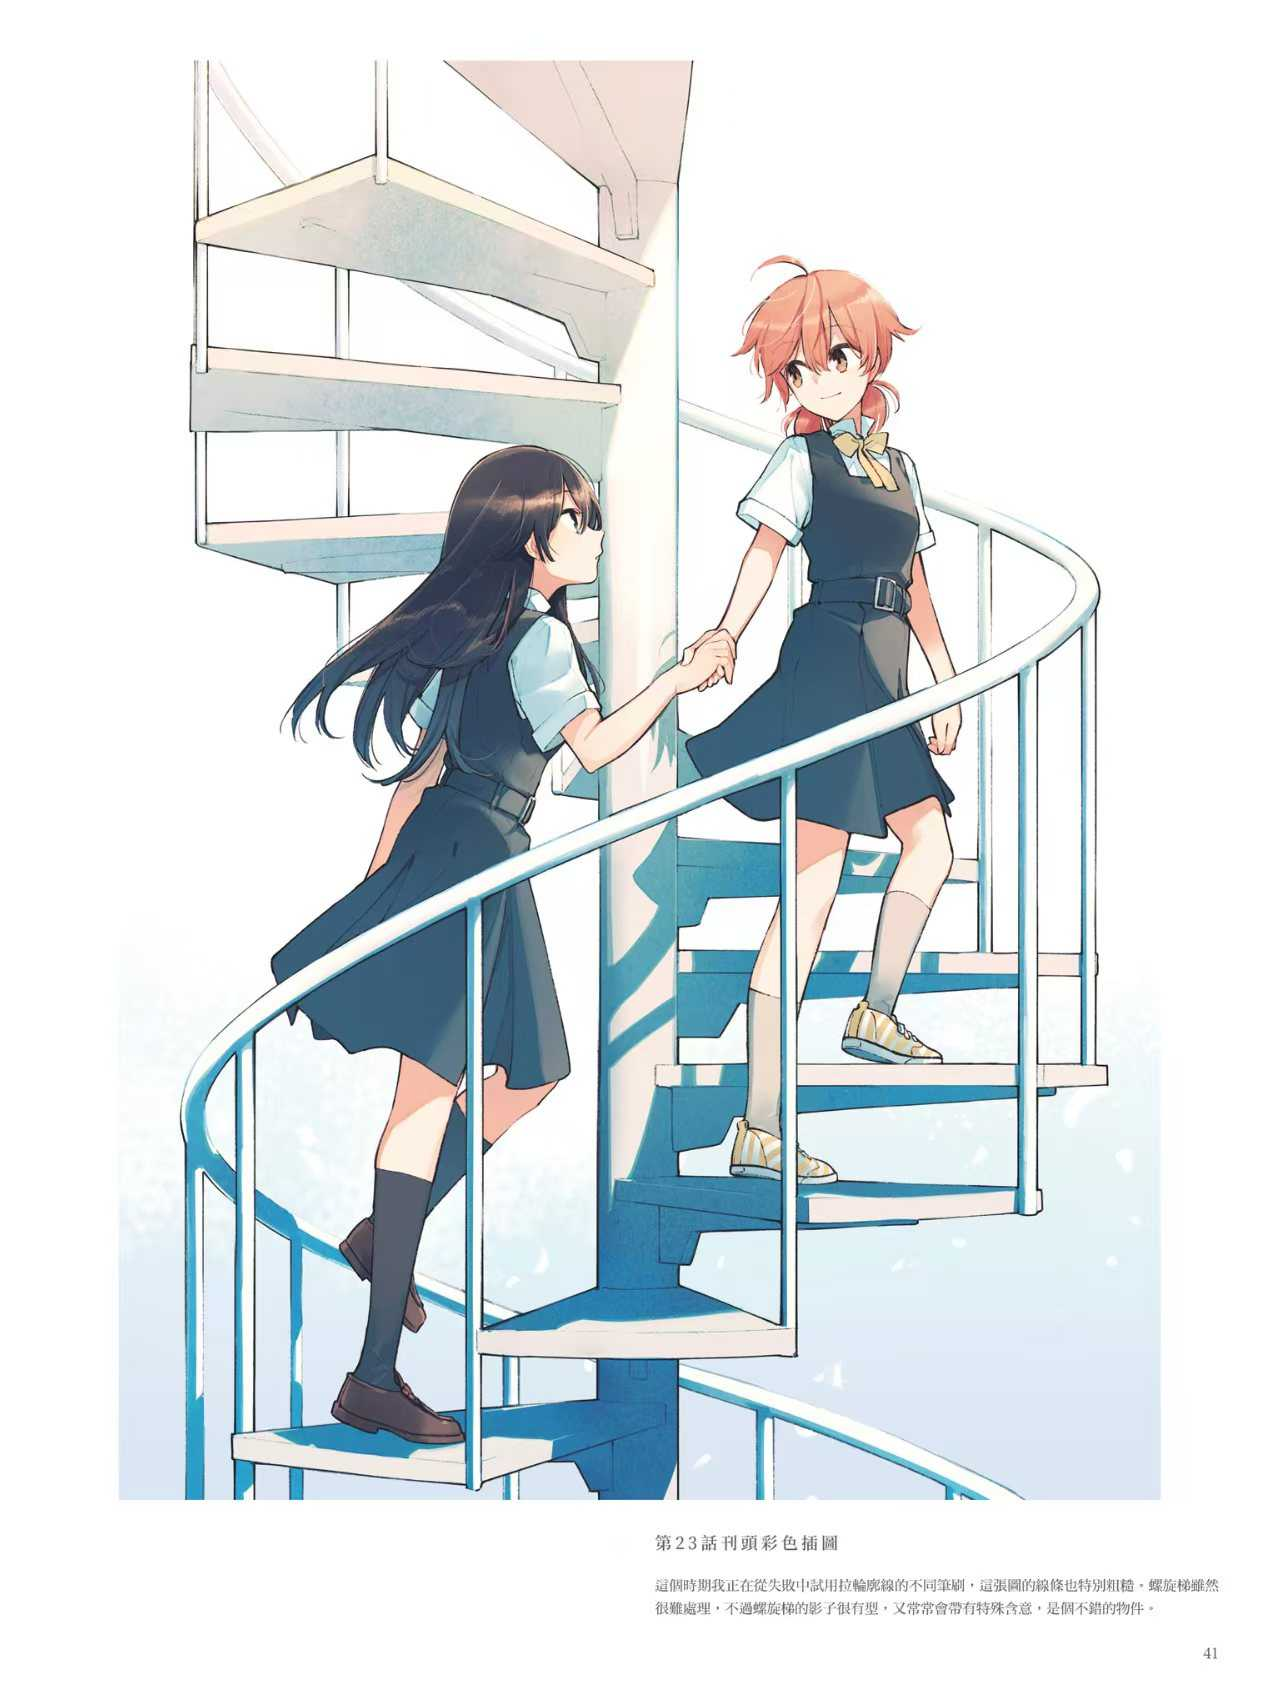
\includegraphics[width=.4\textwidth]{mmexport1748449602397.jpg}}
\caption{双图}\label{fig:双图}
\end{figure} 

\subsection{模型求解}

\textbf{Step1:} 

\textbf{Step2:} 

\textbf{Step3:} 

\subsection{求解结果}

%%%%%%%%%%%%%%%%%%%%%%%%%%%%%%%%%%%%%%%%%%%%%%%%%%%%%%%%%%%%% 

\section{问题三的模型的建立和求解}
\subsection{模型建立}

\subsection{模型求解}

\textbf{Step1:} 

\textbf{Step2:} 

\textbf{Step3:} 

\subsection{求解结果}

%%%%%%%%%%%%%%%%%%%%%%%%%%%%%%%%%%%%%%%%%%%%%%%%%%%%%%%%%%%%% 

\section{问题四的模型的建立和求解}
\subsection{模型建立}

\subsection{模型求解}

\textbf{Step1:} 

\textbf{Step2:} 

\textbf{Step3:} 

\subsection{求解结果}

%%%%%%%%%%%%%%%%%%%%%%%%%%%%%%%%%%%%%%%%%%%%%%%%%%%%%%%%%%%%%

\section{模型的分析与检验}

\subsection{灵敏度分析}

\subsection{误差分析}

%%%%%%%%%%%%%%%%%%%%%%%%%%%%%%%%%%%%%%%%%%%%%%%%%%%%%%%%%%%%%

\section{模型的评价}

\subsection{模型的优点}
\begin{itemize}[itemindent=2em]
\item 优点1
\item 优点2
\item 优点3
\end{itemize}

\subsection{模型的缺点}
\begin{itemize}[itemindent=2em]
\item 缺点1
\item 缺点2
\end{itemize}


\bibliographystyle{gbt7714-numerical}  % 引用格式
\bibliography{ref}  % 引用 ref.bib 文件,无需写 .bib 后缀


\newpage
%%%%%%%%%%%%%%%%%%%%%%%%%%%%%%%%%%%%%%%%%%%%%%%%%%%%%%%%%%%%%
%% 附录
\begin{appendices}
\section{文件列表}
\begin{table}[H]
\centering
\begin{tabularx}{\textwidth}{LL}
\toprule
文件名   & 功能描述 \\
\midrule
example.py & 问题一程序代码 \\
\bottomrule
\end{tabularx}
\label{tab:文件列表}
\end{table}

\section{代码}
\noindent example.py
\lstinputlisting[language=python]{code/example.py}
\end{appendices}

\end{document}
